\documentclass[a4paper, twoside]{report}

\usepackage[english]{babel}
\usepackage[utf8]{inputenc}
\usepackage[T1]{fontenc}
\usepackage{listings}
\usepackage{hyperref}
\hypersetup{colorlinks=false}
\usepackage{lscape}
\usepackage{subfigure}
\usepackage{amsmath}
\usepackage{amssymb}
\usepackage{mathrsfs}
\usepackage{graphicx}
\usepackage[colorinlistoftodos]{todonotes}
\usepackage[backend=biber]{biblatex}

\addbibresource{bibs/references.bib}
%% Sets page size and margins
\usepackage[a4paper,top=3cm,bottom=2cm,left=3cm,right=3cm,marginparwidth=1.75cm]{geometry}

\usepackage{ntheorem}

\theoremstyle{break}
\newtheorem{theorem}{Theorem}[section]
\newtheorem{corollary}{Corollary}[theorem]
\newtheorem{lemma}[theorem]{Lemma}
\newtheorem*{problem}{Problem}[section]
\newtheorem*{architecture}{Architecture}[section]


\DeclareMathOperator{\balance}{balance}
\DeclareMathOperator{\argmin}{argmin}
\DeclareMathOperator{\aggregate}{AGGREGATE}
\DeclareMathOperator{\combine}{COMBINE}
\DeclareMathOperator{\readout}{READOUT}
\DeclareMathOperator{\MAX}{MAX}
\DeclareMathOperator{\MEAN}{MEAN}
\DeclareMathOperator{\relu}{ReLU}
\DeclareMathOperator{\concat}{CONCAT}
\DeclareMathOperator{\mlp}{MLP}
\DeclareMathOperator{\hash}{HASH}
\DeclareMathOperator{\gin}{GIN}


\title{Contemplation on \\
{\it Fair Clustering Through Fairlets}}

\author{Junghyun Lee}
% Update supervisor and other title stuff in title/title.tex

\begin{document}
\begin{titlepage}

\newcommand{\HRule}{\rule{\linewidth}{0.5mm}} % Defines a new command for the horizontal lines, change thickness here

%----------------------------------------------------------------------------------------
%	LOGO SECTION
%----------------------------------------------------------------------------------------


\includegraphics[width=8cm]{title/logo.png}\\[1cm] % Include a department/university logo - this will require the graphicx package
 
%----------------------------------------------------------------------------------------

\center % Center everything on the page

%----------------------------------------------------------------------------------------
%	HEADING SECTIONS
%----------------------------------------------------------------------------------------
\quad\\[1.5cm]
%\textsc{\LARGE MSc Thesis}\\[1.5cm] % Name of your university/college
\textsc{\Large Korea Advanced Institute of Technology}\\[0.5cm] % Major heading such as course name
\textsc{\large Department of Mathematical Sciences}\\[0.5cm] % Minor heading such as course title

%----------------------------------------------------------------------------------------
%	TITLE SECTION
%----------------------------------------------------------------------------------------
\makeatletter
\HRule \\[0.4cm]
{ \huge \bfseries \@title}\\[0.4cm] % Title of your document
\HRule \\[1.5cm]
 
%----------------------------------------------------------------------------------------
%	AUTHOR SECTION
%----------------------------------------------------------------------------------------

\begin{minipage}{0.4\textwidth}
\begin{flushleft} \large
\emph{Author:}\\
\@author % Your name
\end{flushleft}
\end{minipage}
~
\begin{minipage}{0.4\textwidth}
\begin{flushright} \large
\emph{Instructor:} \\
Prof. Chang Dong Yoo 
% Uncomment the following lines if there's a co-supervisor
%\\[1.2em] % Supervisor's Name
%\emph{Co-Supervisor:} \\
%Dr. Adam Smith % second marker's name
\end{flushright}
\end{minipage}\\[3cm]
\makeatother


%----------------------------------------------------------------------------------------
%	DATE SECTION
%----------------------------------------------------------------------------------------

{\large Final Project - Graph}\\[0.5cm]
{\large \emph{EE531: Statistical Learning Theory, Fall 2019}}\\[0.5cm]
{\large \today}\\[2cm] % Date, change the \today to a set date if you want to be precise

\vfill % Fill the rest of the page with whitespace

\end{titlepage}

\begin{abstract}
This writing is an extensive outline of the paper {\it How powerful are graph neural networks?} by Xu {\it et al.}, including summaries of the theorems/lemmas and additional explanation on some of the literatures/points that the paper omitted.

(This is to be accompanied by the pdf file used in the final presentation. Also, the theorem/lemma/corollary numbering is arbitrary, but the statements are exact.)
\end{abstract}

\tableofcontents
\listoffigures

\chapter{Introduction}
This is one of the most important components of the dissertation. It should begin with a clear statement of what the project is about so that the nature and scope of the project can be understood by a lay reader. It should summarise everything you set out to achieve, provide a clear summary of the project's background and relevance to other work and give pointers to the remaining sections of the dissertation which contain the bulk of the technical material.

Further information can be found here: \url{https://goo.gl/k2huN9}.

\section{\LaTeX{} code examples and formatting tips}
Hello, here's a citation \cite{greenwade93}. References are stored in a Bibtex file. Google Scholar and IEEExplore allow you to download citations of papers in Bibtex format from their search engine. Some people use JabRef (\url{http://www.jabref.org}) to manage their database of references.

This is an inline equation $\Gamma(t)=K_i e^{\sin^2(\omega_t)}$. The first paragraph appears without indent but the following ones will have an indentation.

This is an actual named equation:
\begin{equation}
v(x)=\frac{1}{2}\sin(2 \omega t + \phi) e^{-j s t}
\label{eq:cacona}
\end{equation}
\noindent where $\omega$ is the angular speed. Notice that symbols liks $\omega$ should be written in italics whereas measurement units such as V for Volts appear as normal text. This paragraph didn't have an indentation because the first sentence was linked to the definition of equation (\ref{eq:cacona}). A code snippet for an example program is shown in Listing~\ref{lst:code1}.

\begin{lstlisting}[caption=Source code for {\it hello.m},label=lst:code1,breaklines=true,basewidth=4pt,prebreak=**,postbreak=**,frame=single]
for i:=maxint to 0 do
begin
{ do nothing }
end;
Write('Case insensitive ');
Write('Pascal keywords.');
\end{lstlisting}

The characteristic parameters of the system are sumarised in Table~\ref{tab:tab1}. A figure is shown Fig~\ref{fig:felix}, we don't necessarily know if this figure will appear below, above or elsewhere; therefore, the text should never refer to the figure with sentences such as {\it "As shown here:"}.

\begin{figure}[htbp]
\centering

\includegraphics[width=0.3\linewidth]{introduction/fig/Felix_the_cat.pdf}
\caption{Felix the Cat}
\label{fig:felix}
\end{figure}

\begin{table}[htbp]
	\centering
	\begin{tabular}{lll}
		Parameter & Value & Units\\
		\hline
		$P$ & 1 & kW \\
		$Q$ & 0 & kVAr\\
	    \hline
	\end{tabular}
	\caption{Characteristic parameters of the system}
	\label{tab:tab1}
\end{table}

\begin{samepage}
Sometimes, the symbols in an equation are defined as follows\footnote{Some authors like to define their symbols this way.}:
\begin{equation}
	V(t)=A \sin(\omega t+\theta_0)
\end{equation}
\begin{tabular}{lll}
	where & $V$ & is a voltage waveform,\\
	& $A$ & is the amplitude of the voltage,\\
	& $\omega$ & is the angular frequency,\\
	& $t$ & is the time.
\end{tabular}
\end{samepage}

\subsection{A brief comparison between a proper plot and a horrible plot}

Figure \ref{fig:fig2} contains two plots of the same waveform. Subfigure \ref{fig:fig2sub1} shows a badly formatted figure, Subfigure \ref{fig:fig2sub2} shows a much better formatted figure. The problems with Subfigure \ref{fig:fig2sub1}, listed by order or relevance, are the following:

\begin{enumerate}
    \item The font size is too small to be read properly.
    \item The axes aren't labeled properly: the horizontal axis is not labeled and the units of the vertical axis are unknown. Further, symbols must be written in italics whereas numbers and units must be written as normal text.
    \item The choice of limits for the axes is not good, the figure has wide useless empty spaces. The most relevant part of the waveform is the transient that happens between times $t=$0 and $t=$0.05 s, which is less than 10\% of the timespan shown in the figure.
    \item The figure has been scaled without keeping the original aspect ratio and fonts look narrower than they would if the figure had been scaled properly.
    \item The plot doesn't have grid lines. This makes it hard to read the exact value (ie time, voltage) of points in the trace.
    \item The width of the trace is too thin and may not be visible if printed in low resolution.
    \item The choice of units of the vertical axis aren't the best. For example, in this case the plot would be easier to read if voltage had been expressed in kV instead of V.
    \item The figure was exported as a bitmap (e.g. png, jpg, bmp) instead of being exported in vector format (e.g. eps, svg, pdf) and visual artifacts appear when the figure is scaled up or down in order to fit in the document.
\end{enumerate}

\begin{figure}[htbp]
	\centering
	\subfigure[A horrible one.]{
		\label{fig:fig2sub1}
        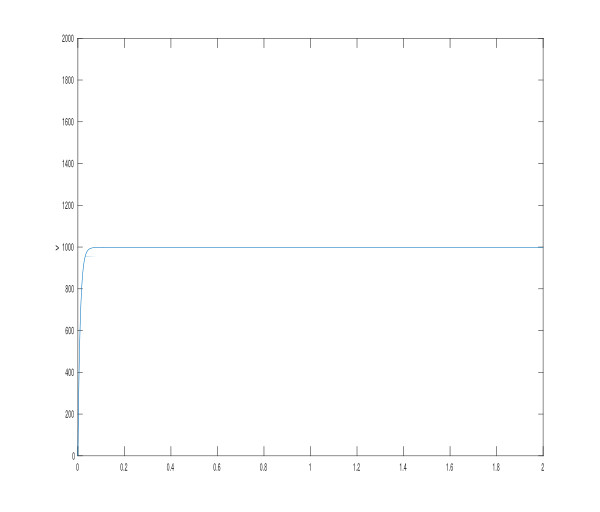
\includegraphics[width=0.5\linewidth]{introduction/fig/figure1.jpg}}
	\subfigure[A proper one.]{
		\label{fig:fig2sub2}
		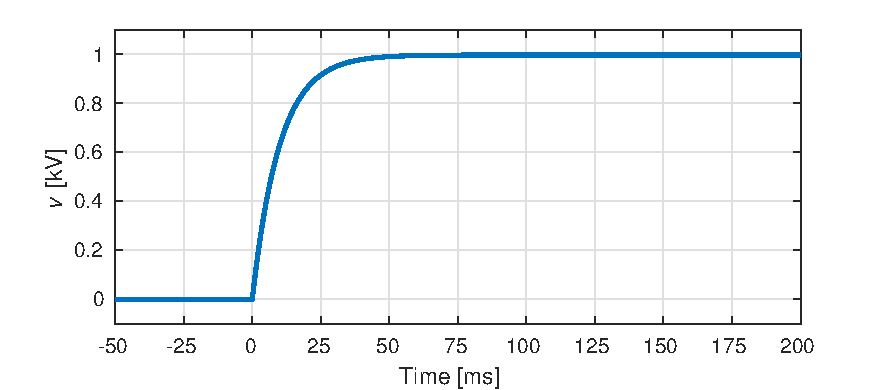
\includegraphics[width=0.6\linewidth]{introduction/fig/figure2.pdf}}
	\caption{A figure with two subfigures.}
	\label{fig:fig2}
\end{figure}

\begin{landscape}
	\begin{figure}[htbp]
\centering

\includegraphics[width=0.5\linewidth]{introduction/fig/Felix_the_cat.pdf}
\caption{Here's a large drawing of Felix the Cat that wouldn't fit in a portrait page}
\label{fig:felix2}
\end{figure}
\end{landscape}

\section{Objectives}
\section{Challenges}
\section{Contributions}
\chapter{Preliminaries}

\section{GNNs}

Consider a graph, $G = (V, E)$, or a data with graph structure. Then each node $v \in V$ is associated with a {\it node feature vector}, denoted as $X_v$.
There are two tasks of interest where GNN is commonly used:

\begin{problem}[Node Classification Problem]
Each $v \in V$ has an associated label $y_v$.

\noindent{\bf Goal:} Learn a representation vector $h_v$ of $v$ such that $y_v = f(h_v)$ i.e. such that $v$'s label can be predicted.
\end{problem}


\begin{problem}[Graph Classification Problem]
A set of graphs $\{G_1, \dots, G_N\} \subset \mathcal{G}$ is given, along with their labels $\{y_1, \dots, y_N\} \subset \mathcal{Y}$.

\noindent{\bf Goal:} Learn a representation vector $h_G$ of $G$ such that $y_G = f(h_G)$ i.e. such that $G$'s label can be predicted. 
\end{problem}


Modern GNNs follow a {\bf neighborhood aggregation strategy} (message passing strategy) in which it iteratively updates the representation of a node by aggregating representations of its neighbors.

Denote $h_v^{(k)}$ as the feature vector of node $v$ at the $k$-th iteration/layer, and let us initialize it as $h_v^{(0)} = X_v$.
Then in this framework, the $k$-th layer of a GNN can be written as

	$$a_v^{(k)} = \aggregate^{(k)} \left( \left\{ h_u^{(k - 1)} : u \in \mathcal{N}_G(v) \right\} \right)$$
	$$h_v^{(k)} = \combine^{(k)} \left( h_v^{(k - 1)}, a_v^{(k)} \right)$$

Different choices of $\aggregate^{(k)}$ and $\combine^{(k)}$ have led to different GNN variants/architectures.

\begin{architecture}[GraphSAGE\cite{Hamilton2017}]
	$$a_v^{(k)} = \MAX \left( \left\{ \relu \left( W h_u^{(k - 1)} \right) : u \in \mathcal{N}_G(v) \right\} \right)$$
	$$h_v^{(k)} = W \left[ h_v^{(k - 1)}, a_v^{(k)} \right]$$
\end{architecture}

\begin{architecture}[Graph Convolutional Networks(GCN)\cite{Kipf2017}]
	$$h_v^{(k)} = \relu \left( W \MEAN \left\{ h_u^{(k - 1)} : u \in \mathcal{N}_G(v) \cup \{v\} \right\} \right)$$
\end{architecture}


Observe that for node classification tasks, the final node representation $h_v^{(K)}$ is directly used for prediction.
However for graph classification tasks, this is not the case i.e. some additional work has to be done to "process" the final node representation to obtain the entire graph's representation.
This is done by aggregating the final node representations by $\readout$ function:
	$$h_G = \readout \left( \left\{ h_v^{(K)} : v \in V \right\} \right)$$ 
	
($\readout$ can be a simple permutation invariant function, or something more sophisticated\cite{Ying2018}\cite{Zhang2018})

%---------------------------------------------------------

\section{WL test}

Now consider the following problem:

\begin{problem}[\textsc{Graph Isomorphism (GI)}]
{\bf Input}:  Two finite graphs $G_1$ and $G_2$

\noindent{\bf Question}: $G_1 \cong G_2$?
\end{problem}

This ubiquitous problem appears everywhere: from mathematical logic, theory of computation, machine learning, to seemingly unrelated fields such as computer vision.
And this seemingly harmless problem has harassed researchers for decades!


It is currently known that \textsc{GI} can be solved in quasipolynomial time {\it i.e.} in $O \left( 2^{O \left( \left( \log n \right)^c \right)} \right) (c > 0)$ time\cite{Babai2016}.
The precise statement is as follows:
	
\begin{theorem}[Babai, 2015]
The Graph Isomorphism problem ... can be solved in quasipolynomial time.
\end{theorem}

But this is not practical.
In practice, other less efficient algorithms are used, such as algorithms by McKay (1981), Schmidt \& Druffel (1976), Ullman (1976)...etc.


Here, we shall talk about one specific combinatorial algorithm for \textsc{GI}: the Weisfeiler-Lehman test of graph isomorphism\cite{Weisfeiler1968}, or simply WL test.

WL test is proved to be successful (and computationally efficient) in isomorphism testing for a broad class of graphs\cite{Babai1979} There are some (corner) cases (ex. regular graphs) when the WL test fails\cite{Cai1992}.

The reason the people working on GNNs got so interested in the WL test is that its 1-dimensional form (a.k.a. "na\"ive vertex refinement") is {\it based on neighbor aggregations}, analogous to the GNNs!
(And that is why we'll be focused only on the 1-dim case)

Let $(G, l)$ be a labeled graph i.e. a graph $G$ with an endowed node coloring $l : V(G) \rightarrow \Sigma$.
($\Sigma$: arbitrary codomain)
Here is the full algorithm for the 1-dim WL test\cite{Shervashidze2009}:

\begin{figure}[hbt]
	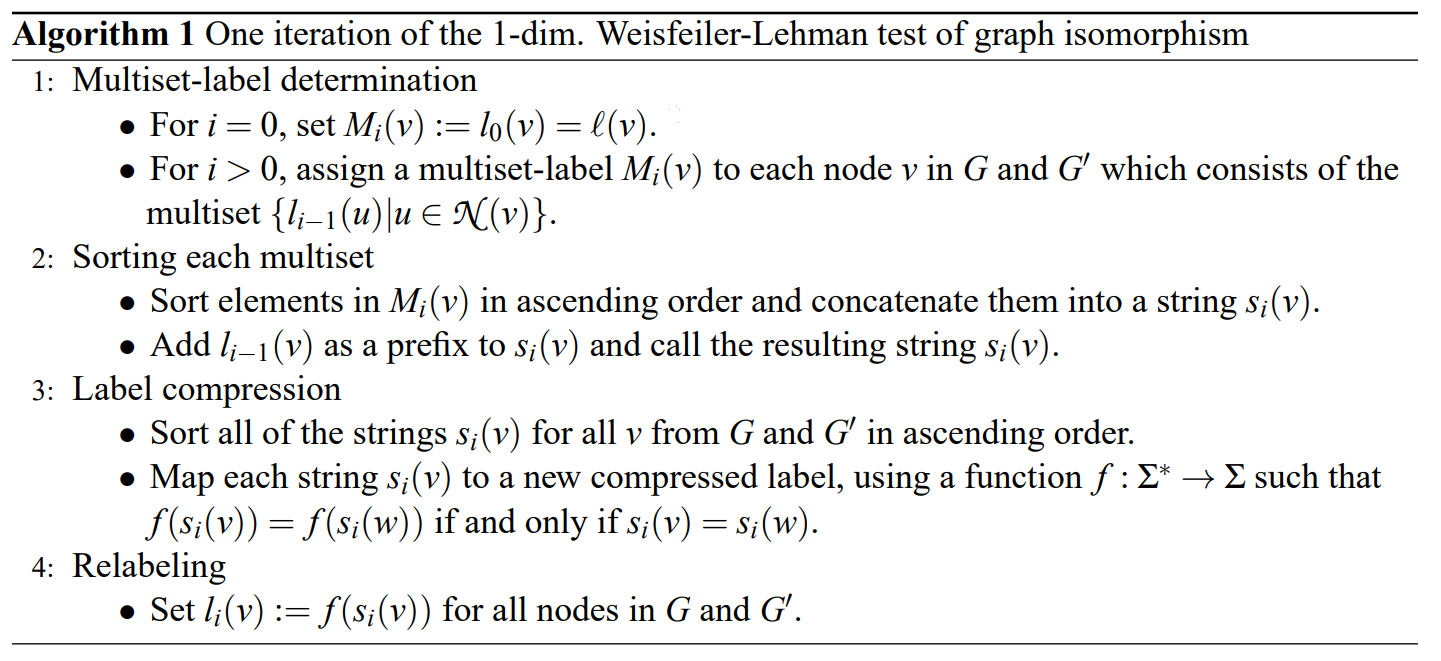
\includegraphics[height=7cm]{preliminaries/fig/wl-alg.png}
	\caption{One iteration of 1-dim WL test}
\end{figure}
	(This why this 1-dim version is commonly called the {\it color refinement algorithm})

To relate this to GNN, we need one more concept; graph kernel.

Graph kernel is a kernel function that defines {\it inner product on graphs} \cite{Vishwanathan2010}.
Intuitively, it is a function that measures the similarity of a pair of two given graphs.
There are many different variants of graph kernels, but we'll be focused on the Weisfeiler-Lehman subtree kernel\cite{Shervashidze2009}.
(Refer to \cite{Vishwanathan2010} for a extensive study of graph kernels and \cite{Shervashidze2011} for a more thorough explanation of the WL subtree kernel)

The WL subtree kernel counts common {\it original and compressed labels} i.e. common multiset strings in two graphs, resulting from 1-dim WL test.
Below shows the algorithm for calculating the WL subtree kernel:

\begin{figure}[hbt]
	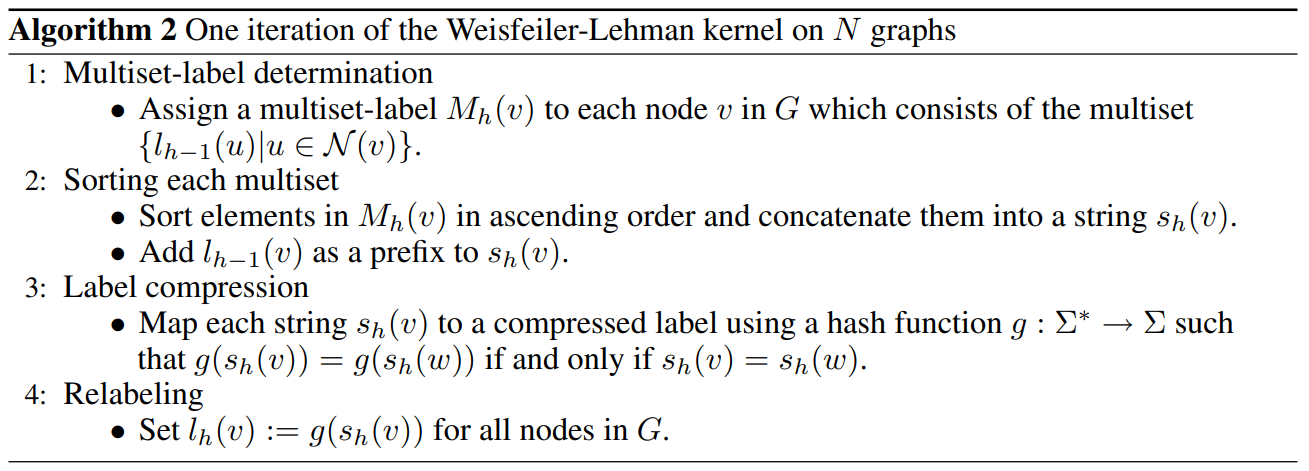
\includegraphics[height=6cm]{preliminaries/fig/wl-kernel-alg.png}
	\caption{One iteration of WL subtree kernel}
\end{figure}

And below figure is a visualization of one run of the WL subtree kernel:

\begin{figure}[hbt!]
\centering
	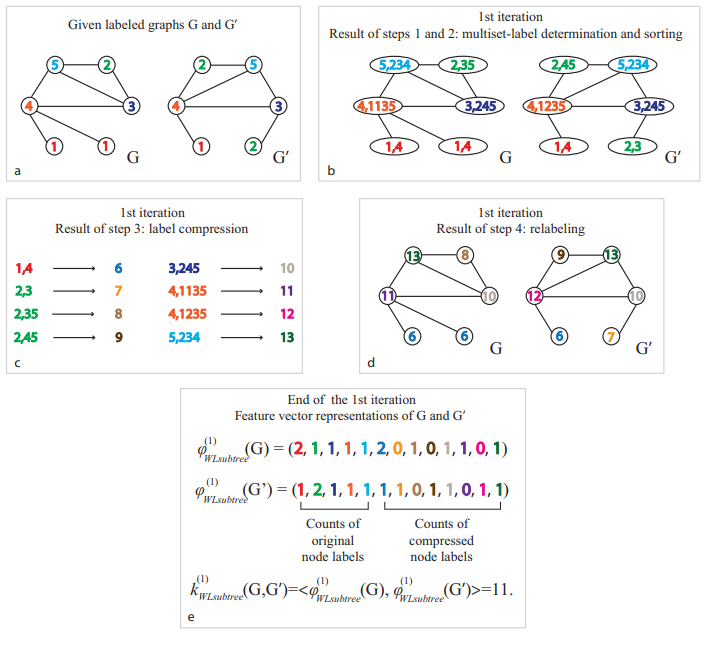
\includegraphics[height=13cm]{preliminaries/fig/fig1.png}
	\caption{Illustration of the computation of the WL subtree kernel (with respect to one iteration) for two graphs}
\end{figure}

\newpage
\section{(Overview of) Theoretical Framework}

In other words, the WL subtree uses the counts of node labels at different iterations of the WL test as the feature vector of a graph.
Intuitively, a node’s label at the $k$-th iteration of the 1-dim WL test represents a {\bf subtree structure of height k rooted at the node}.

Thus, the graph features considered by the WL subtree kernel are essentially counts of different rooted subtrees in the graph!

\begin{figure}[hbt!]
\centering
	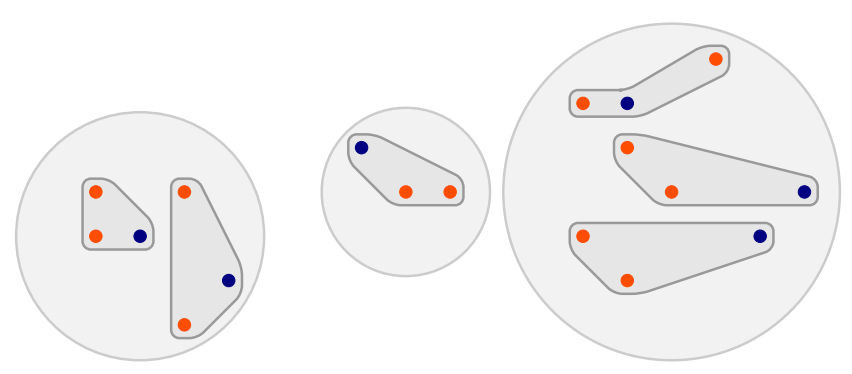
\includegraphics[height=4cm]{preliminaries/fig/fig2.png}
	\caption{An overview of the theoretical framework}
\end{figure}

What this tells us is that if a GNN's aggregation function captures the {\it full multiset} of node neighbors, the GNN can capture the rooted subtrees in a recursive manner and be as powerful as the WL test (as shown in above figure).

To analyze the representational power of a GNN, we ask ourselves the question: {\it when does a GNN map two nodes to the same location in the embedding space)? }
{\bf Intuitively, a maximally powerful GNN maps two nodes to the same location only if they have identical subtree structures with identical features on the corresponding nodes.}
Since subtree structures are defined recursively via node neighborhoods (above figure), we can reduce our analysis to the question whether a GNN maps two neighborhoods (i.e., two multisets) to the same embedding or representation.
A maximally powerful GNN would never map two different neighborhoods, i.e., multisets of feature vectors, to the same representation.
This means its aggregation scheme must be injective. Thus, we abstract a GNN’s aggregation scheme as a class of functions over multisets that their neural networks can represent, and analyze whether they are able to represent injective multiset functions.

(Above paragraph is taken directly from the paper because it is the key point in this whole work!)

\chapter{Results}
%For my evaluation, I've used {\bf Tensorboard} for plotting the learning(loss) curve and performance(accuracy) curve for both training and validating processes. Also, I've used external open source library({\bf pretty-print-confusion-matrix}\footnote{\url{https://github.com/wcipriano/pretty-print-confusion-matrix}}) for plotting the confusion matrix for the test set.
Here,
\begin{itemize}
\item Original model: One with uniform initialization with dropouts(rate=0.5).

\item Ver. 1: Original model with Xavier (Uniform) Initialization

\item Ver. 2: Original model without dropouts

\item Ver. 3: Original model with Xavier Initialization and without dropouts
\end{itemize}

In all the plots, x-axis corresponds to the epoch.
As for the graphs,

\begin{itemize}
\item Accuracy graph
	\begin{itemize}
	\item Dark red: train accuracy
	\item Bright red: validation accuracy
	\end{itemize}

\item Loss graph
	\begin{itemize}
	\item Dark blue: train loss
	\item Bright blue: validation loss
	\end{itemize}
\end{itemize}

\newpage
\section{Original model}

\begin{figure}[htbp]
\centering
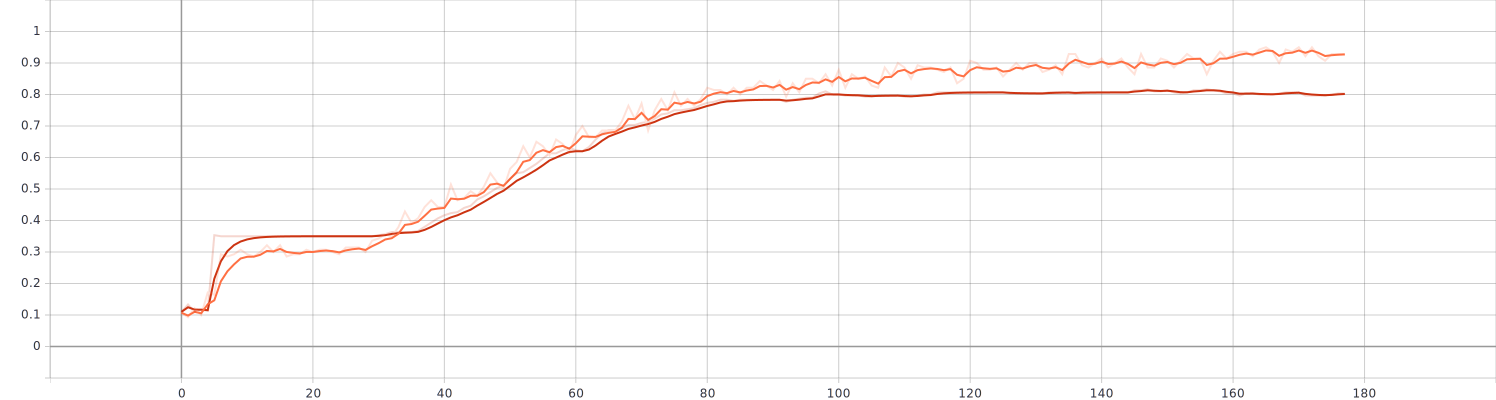
\includegraphics[width=0.7\linewidth]{results/fig/Accuracy0.png}
\caption{Accuracy graph}
\label{fig:accuracy0}
\end{figure}

\begin{figure}[htbp]
\centering
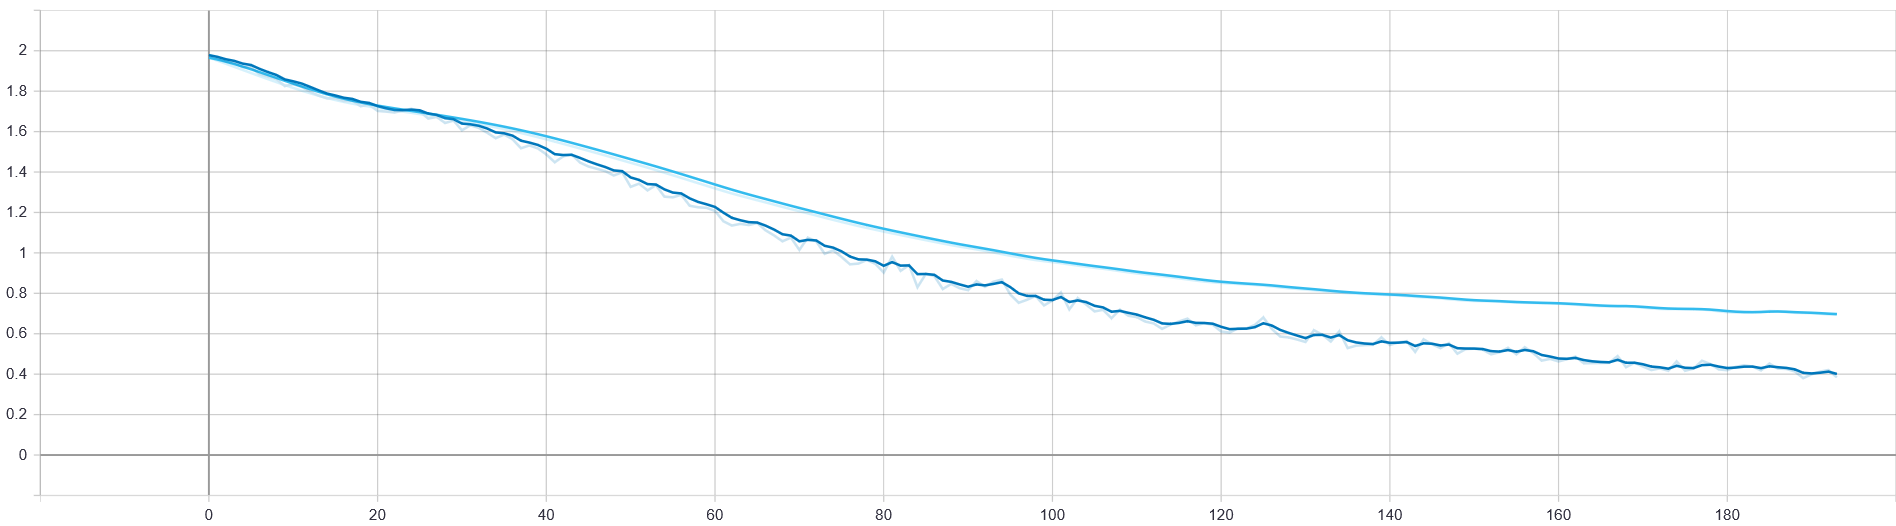
\includegraphics[width=0.7\linewidth]{results/fig/Loss0.png}
\caption{Loss graph}
\label{fig:evaluation0}
\end{figure}

\begin{figure}[htbp]
\centering
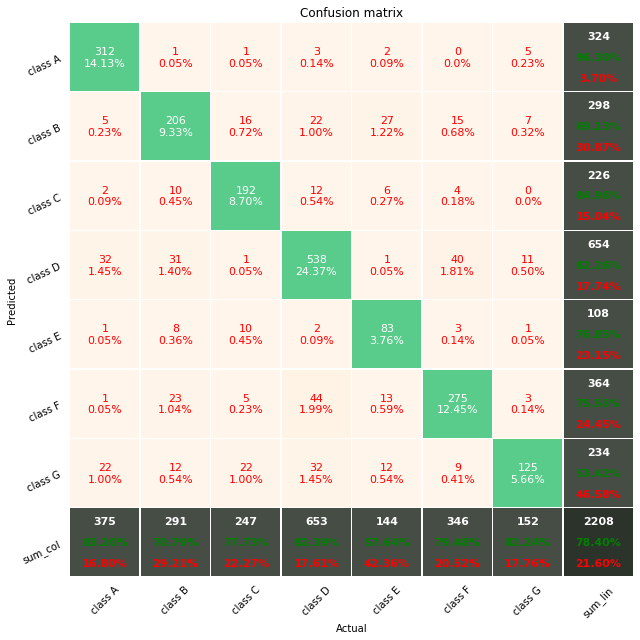
\includegraphics[width=0.6\linewidth]{results/fig/confusion0.png}
\caption{Confusion matrix}
\label{fig:confusion0}
\end{figure}

\newpage
\section{Modified Model (Ver. 1)}

\begin{figure}[htbp]
\centering
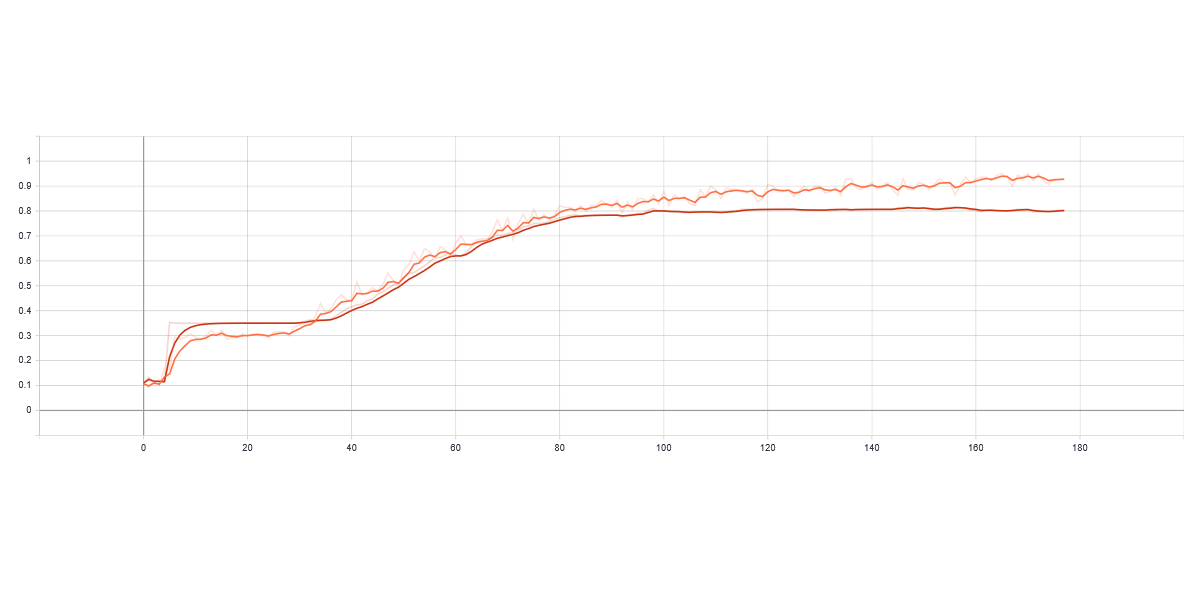
\includegraphics[width=0.7\linewidth]{results/fig/Accuracy1.png}
\caption{Accuracy graph}
\label{fig:accuracy1}
\end{figure}

\begin{figure}[htbp]
\centering
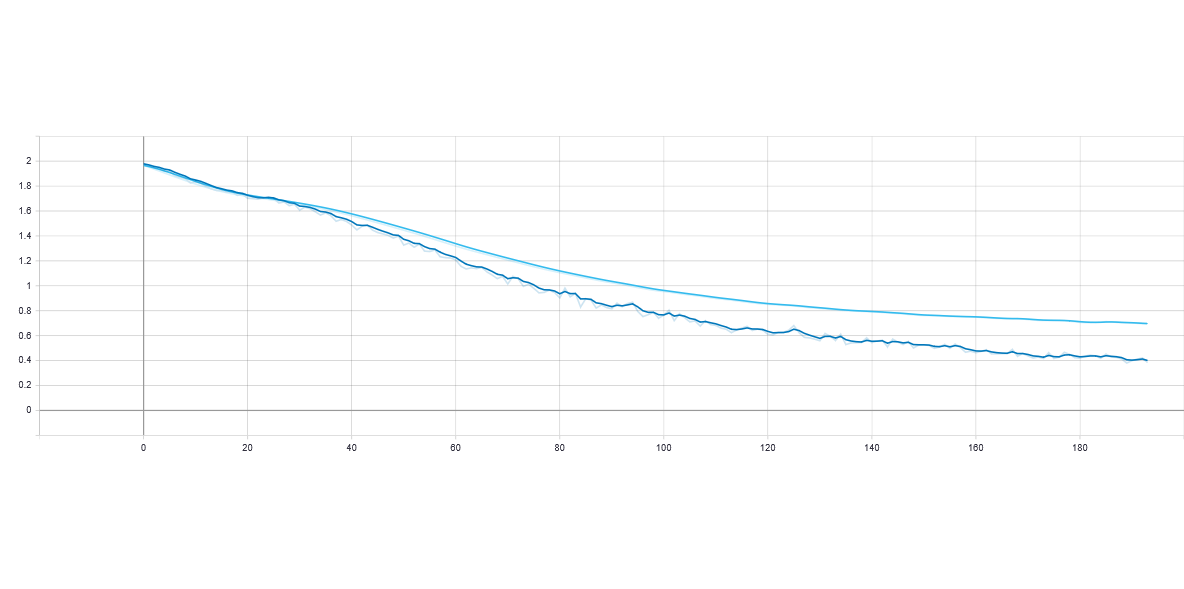
\includegraphics[width=0.7\linewidth]{results/fig/Loss1.png}
\caption{Loss graph}
\label{fig:evaluation1}
\end{figure}

\begin{figure}[htbp]
\centering
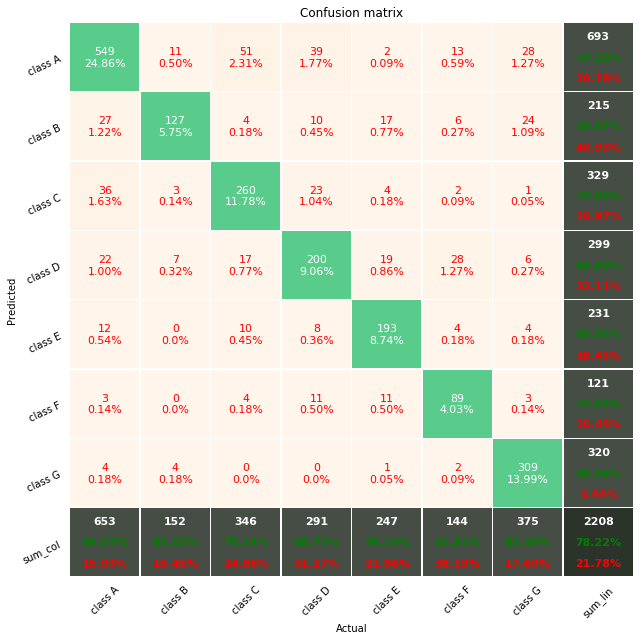
\includegraphics[width=0.6\linewidth]{results/fig/confusion1.png}
\caption{Confusion matrix}
\label{fig:confusion1}
\end{figure}

\newpage
\section{Modified Model (Ver. 2)}

\begin{figure}[htbp]
\centering
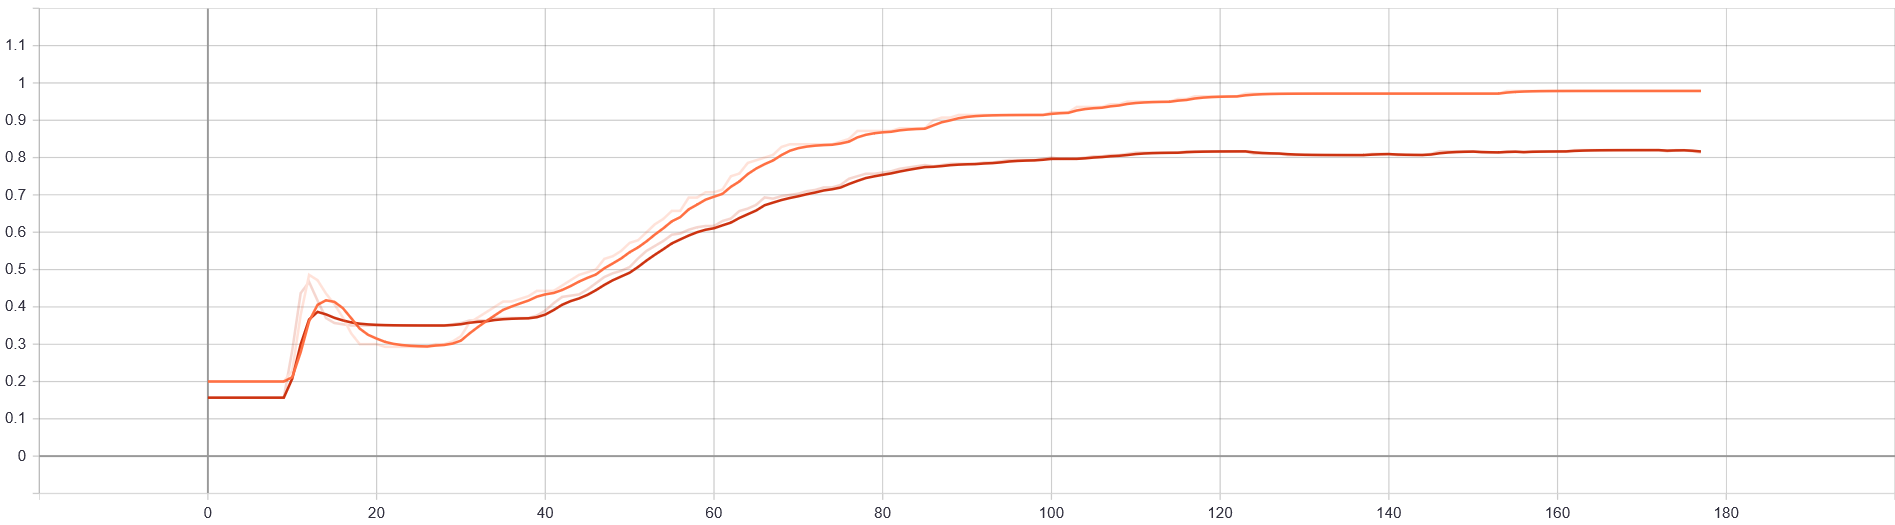
\includegraphics[width=0.7\linewidth]{results/fig/Accuracy2.png}
\caption{Accuracy graph}
\label{fig:accuracy2}
\end{figure}

\begin{figure}[htbp]
\centering
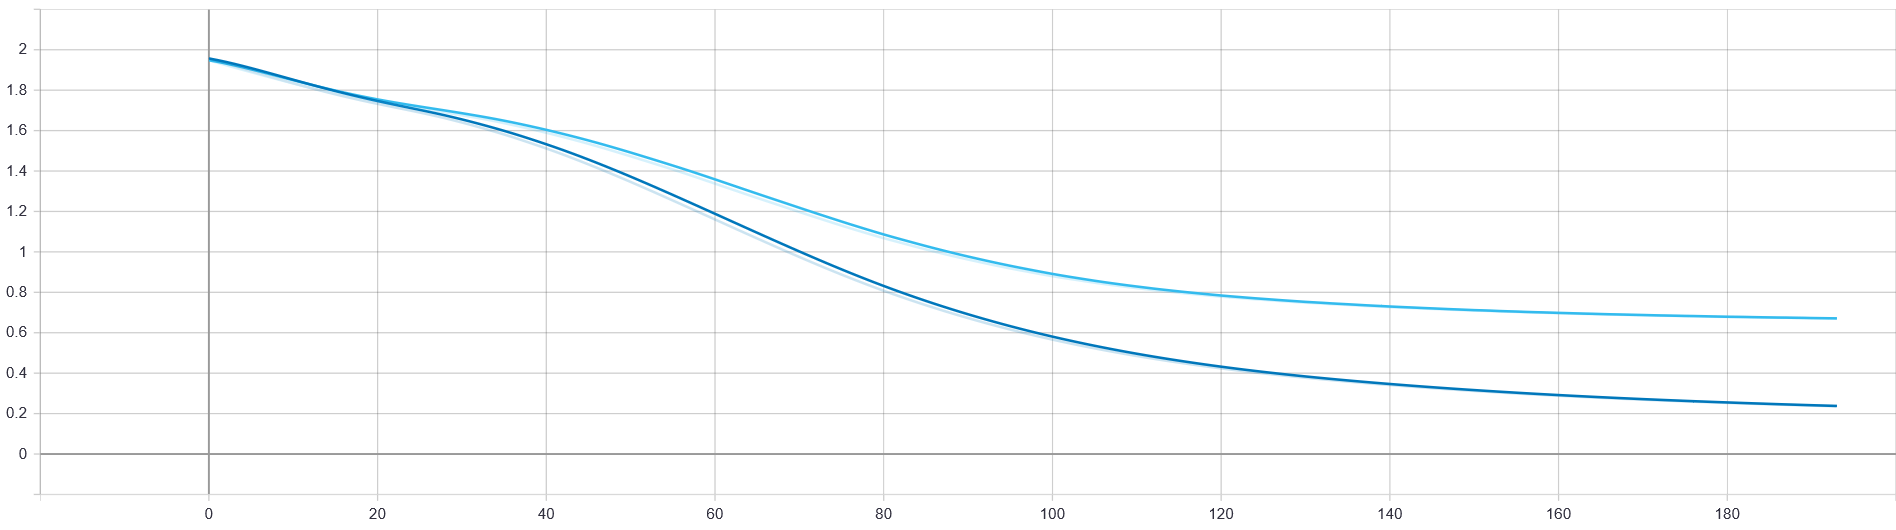
\includegraphics[width=0.7\linewidth]{results/fig/Loss2.png}
\caption{Loss graph}
\label{fig:evaluation2}
\end{figure}

\begin{figure}[htbp]
\centering
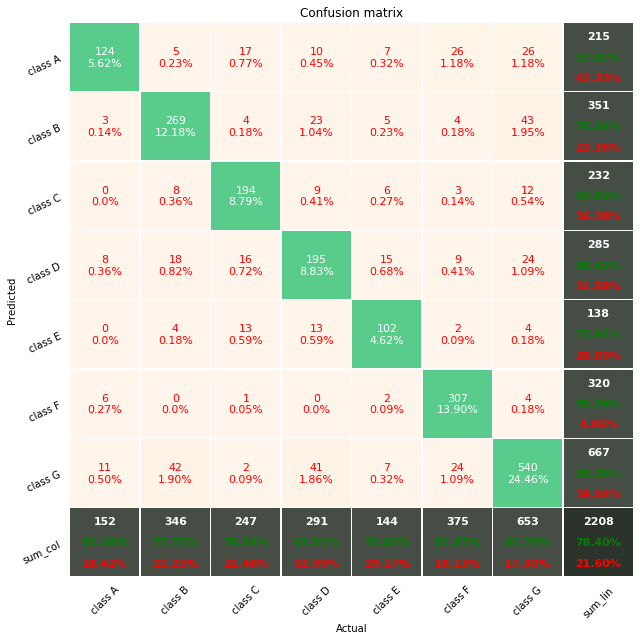
\includegraphics[width=0.6\linewidth]{results/fig/confusion2.png}
\caption{Confusion matrix}
\label{fig:confusion2}
\end{figure}

\newpage
\section{Modified Model (Ver. 3)}

\begin{figure}[htbp]
\centering
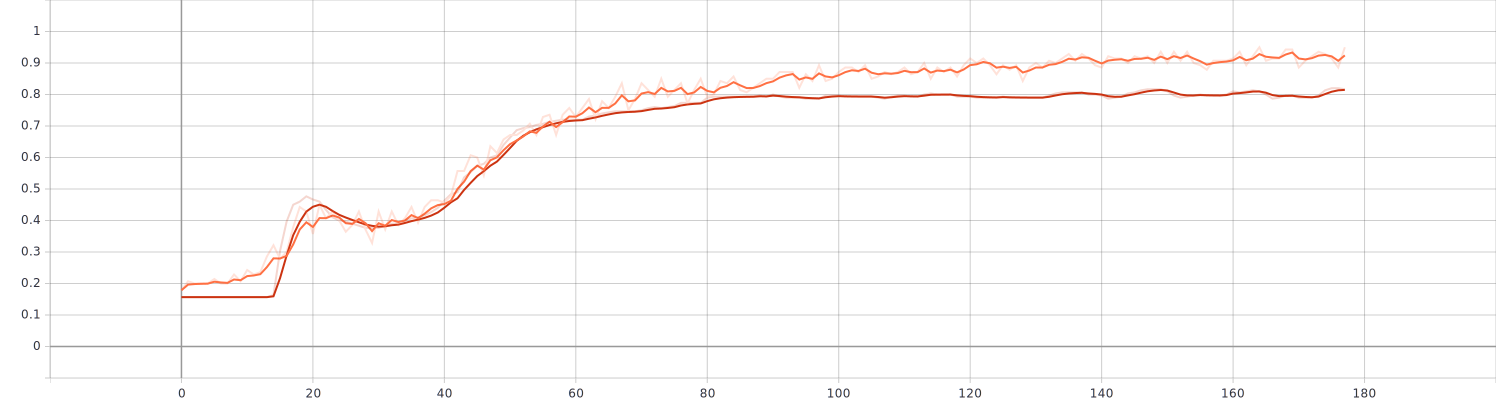
\includegraphics[width=0.7\linewidth]{results/fig/Accuracy3.png}
\caption{Accuracy graph}
\label{fig:accuracy3}
\end{figure}

\begin{figure}[htbp]
\centering
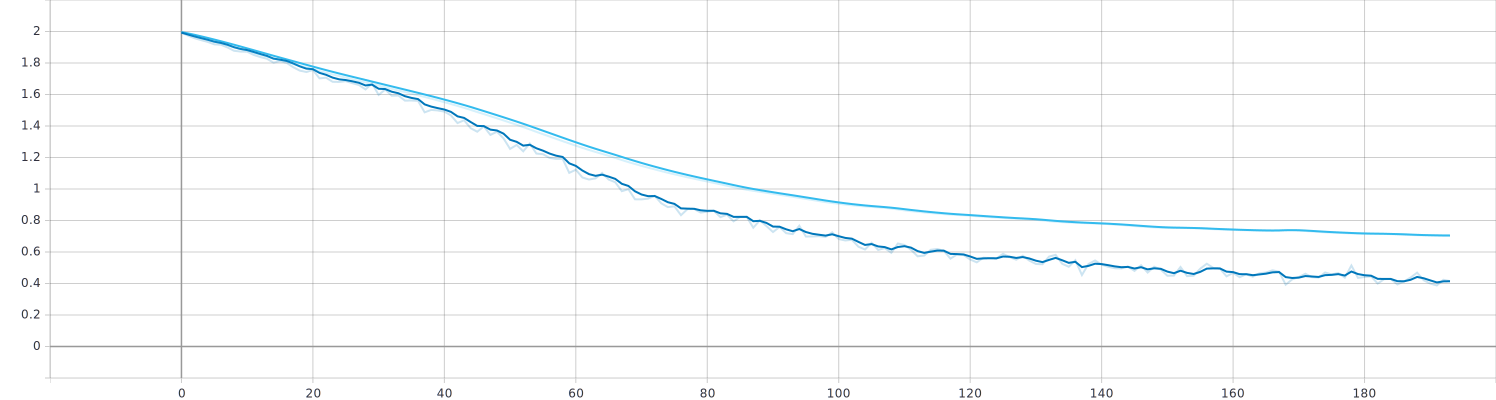
\includegraphics[width=0.7\linewidth]{results/fig/Loss3.png}
\caption{Loss graph}
\label{fig:evaluation3}
\end{figure}

\begin{figure}[htbp]
\centering
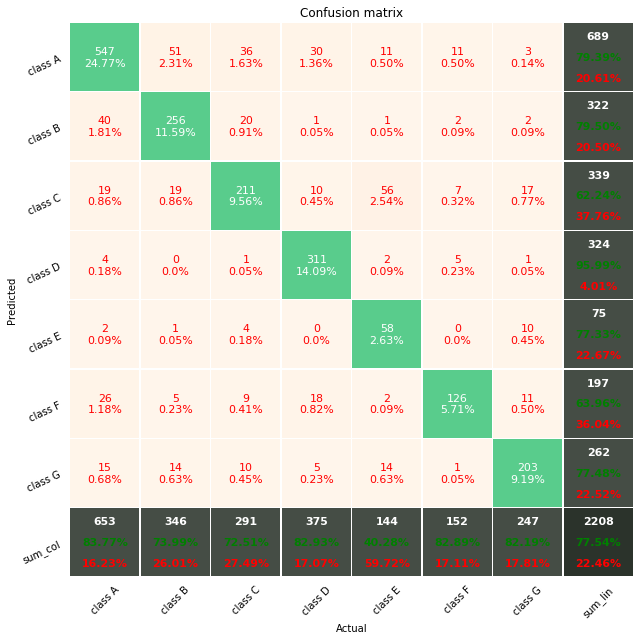
\includegraphics[width=0.6\linewidth]{results/fig/confusion3.png}
\caption{Confusion matrix}
\label{fig:confusion3}
\end{figure}

\chapter{Experiments}

The goal of the experiments is two-fold:

\begin{itemize}
	\item Show that the traditional algorithms for $k$-center and $k$-median tend to produce unfair clusters

	\item Show that the proposed algorithm outputs clusters that respect the fairness guarantees
\end{itemize}


\section{Experiment Design}

3 datasets from \cite{Lichman2013} were used:
\begin{itemize}
	\item Diabetes (gender)
	\item Bank (married or not married)
	\item Sensus (gender)
\end{itemize}

The atttributes in the parenthesis are the protected attributes for each one. The unprotected attributes were chosen as the numeric attributes such as age, capital-gain...etc. (different for each dataset)

As for the algorithm, the flow-based fairlet decomposition algorithm (as discussed previously) was implemented.
For the vanilla $k$-center clustering algorithm, the {\it greedy furthest point algorithm\cite{Gonzalez1985}} was used.
For the vanilla $k$-median clustering algorithm, {\it single swap algorithm\cite{Arya2004}} was used. The reason for this choice, even though it obtains 5-approximation in the worst case, is that it performs well in practice. (Refer to Kanungo {\it et al.}, 2002) for more information.)

In all cases, the experiment was done with $t' = 2$ i.e. aiming for balance of at least $0.5$ in each cluster.

\newpage
\section{Results / Analysis}

\begin{figure}[hbt!]
\centering
  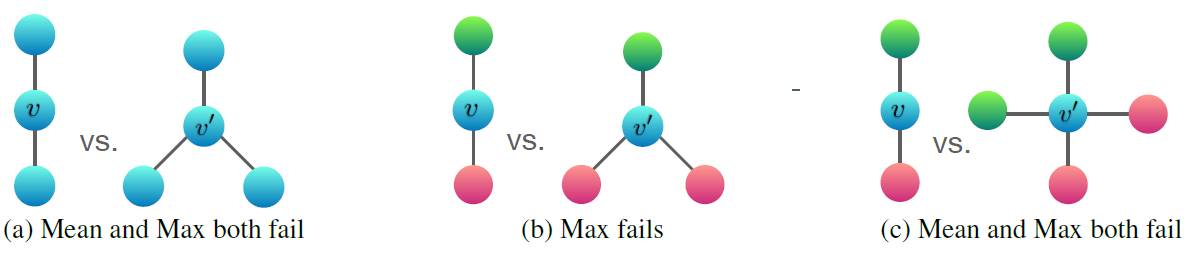
\includegraphics[height=7cm]{experiments/fig/fig4.png}
  \caption{Empirical performance of the classical and fair clustering median and center algorithms on the three datasets. The cost of each solution is on left axis, and its balance on the right axis.}
\end{figure}

Observe that as expected, the balance of the solutions produced by the classical algorithms is very low. More than half of the cases show the phenomenon of balance being at 0 for high value of $k$.

On the other hand the fair clustering solutions maintain a balanced solution, regardless of the value of $k$. Not surprisingly, the balance comes with a corresponding increase in cost, and the fair solutions are costlier than
their unfair counterparts.
In all of the scenarios the overall cost of the clustering converges
to the cost of the fairlet decomposition, which serves as a lower bound on the cost of the optimal solution.
\chapter{Conclusion}
%\appendix
\chapter{First Appendix}
The appendices contain information which is peripheral to the main body of the dissertation. Information typically included are things like program listings, complex circuit diagrams, tables, proofs, graphs or any other material which would break up the theme of the text if it appeared in situ.

%1. Note that being powerful entails “being able to” map nodes with different subtrees to different representations. If a model is not capable of achieving this, then it’s intrinsically less powerful in distinguishing different graphs. In addition, to combat noise, we can simply regularize the mapping function to be locally smooth (e.g., by using Virtual Adversarial Training [1]). Nonetheless, in many graph classification applications including those in our experiments, the node features have specific meanings (e.g. an atom of certain types) and are not noisy.


\printbibliography
%\bibliographystyle{unsrt}
%\bibliography{bibs/references}
\addcontentsline{toc}{chapter}{Bibliography}

\end{document}